%%%%%%%%%%%%%%%%%%%%%%%%
%
% $Autor: Manoj Kumar Prabhakaran $
% $Datum: 2025-03-06 $
% $Pfad: GitHub/ML24-EX03-Pico4MLPro/Pico4MLPro/Contents/General/ApplicationMagicWand.tex $
% $Version: 1 $
%
%%%%%%%%%%%%%%%%%%%%%%%%











\chapter{Domain Knowledge: Magic Wand with an Arducam Pico4ML-Pro}



\section{Application}

The Magic Wand application harnesses the Arducam Pico4ML-Pro, a compact RP2040-based development board featuring a 2.4-inch LCD screen, built-in camera, microphone, and multiple Mega SPI camera adapters, optimized for machine vision and TinyML tasks \cite{Arducam:2023}. This device integrates inertial measurement units (IMUs) and visual sensors to enable real-time gesture recognition, transforming the wand into an interactive tool for applications such as gaming, assistive technology, or human-computer interaction. The RP2040’s dual-core ARM Cortex-M0+ processors, operating at up to 133 MHz, provide limited computational power (approximately 264 DMIPS), necessitating highly optimized ML models for low-latency, energy-efficient operation on the edge \cite{rub:2022}. The integration of IMUs (accelerometer and gyroscope) and a camera aligns with state-of-the-art edge AI systems, as described in recent studies on low-power wearables and embedded vision \cite{Banerjee:2023, Vectornav:2021}.



\section{Problem Definition}

The core technical challenge is designing a gesture recognition system on the resource-constrained Arducam Pico4ML-Pro that achieves high accuracy, low latency, and minimal power consumption. Specific gestures—such as the "Wings" (a side-to-side W-shaped motion), "Ring" (a circular hand motion), "Slope" (a diagonal upward or downward sweep), and custom user-defined patterns—must be detected reliably under varying conditions, including different user speeds, orientations, and environmental noise. This requires addressing several technical hurdles: (1) the limited memory (264 KB SRAM) and storage (2 MB flash) of the RP2040, (2) the trade-off between model complexity and inference speed, and (3) robustness against sensor noise, user variability, and real-world dynamics. Recent research highlights similar challenges in IMU-based gesture control for low-power devices, emphasizing the need for lightweight algorithms like quantized neural networks or decision trees \cite{Perumandla:2021, Garcia:2019, Sadiq:2022}.



\section{Data Acquisition}

Data acquisition for the Magic Wand involves collecting multimodal sensor data from the Pico4ML-Pro’s IMU (accelerometer, gyroscope) \cite{Din:2020} and camera, processed in real-time on the edge. The IMU captures three-dimensional acceleration and angular velocity at high sampling rates (e.g., 100 Hz), providing temporal data on motion trajectories. The camera, with its Mega SPI interface, captures visual frames of hand movements, which are processed for spatial and temporal features. For gesture detection, datasets are prepared by recording sequences of movements, such as:



\begin{itemize}

	\item \textbf{Wings Gesture (W)}: A side-to-side W-shaped motion, typically executed at varying speeds, requiring IMU data to capture acceleration peaks and angular changes, and visual data to track hand position.

	\item \textbf{Ring Gesture}: A circular hand motion, detected through consistent angular velocity patterns in the IMU and circular trajectories in camera frames.

	\item \textbf{Slope Gesture}: A diagonal upward or downward sweep, identified by linear acceleration trends and spatial displacement in both IMU and visual data.

	\item \textbf{Custom Gestures}: User-defined patterns, such as zigzag or spiral motions, requiring flexible data collection protocols to accommodate variability.

\end{itemize}



\begin{figure}[H]\centering

	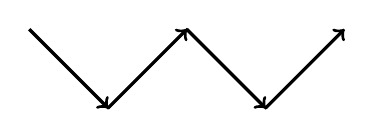
\begin{tikzpicture}

		% define point

		\coordinate (A)  at (1, 1);

		\coordinate (O)  at (2, 0);

		\coordinate (B)  at (3, 1);

		\coordinate (C)  at  (4,0);

		\coordinate (D) at  (5,1);

		% angle  

		\draw[thick] (A) -- (O) -- (B) -- (C)-- (D);

		%	\draw pic[draw=black,eccentricity=2.9]

		%\pic [draw,"$\alpha_1$",angle radius=20,->,angle eccentricity=1.4]

		%  {angle = B--O--A};

		\draw [->, very thick] (1,1) -- (2,0)  node [midway, above] {\scriptsize };

		\draw [->, very thick] (2,0) -- (3,1)  node [midway, above] {\scriptsize };

		\draw [->, very thick] (3,1) -- (4,0)  node [midway, above] {\scriptsize };

		\draw [->, very thick] (4,0) -- (5,1)  node [midway, above] {\scriptsize };

	\end{tikzpicture}

	\captionof{figure}{\textbf{Wing Gesture \cite{Warden:2020}}}

	\label{fig:Wing Gesture}

\end{figure}



\begin{figure}[H]\centering

	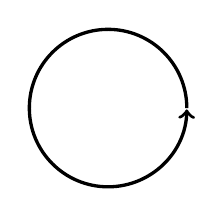
\begin{tikzpicture}

		\draw[->,very thick] (0,0) arc[radius=1cm,start angle=0,delta angle=359];

	\end{tikzpicture}

	\captionof{figure}{\textbf{Ring Gesture \cite{Warden:2020}}}

	\label{fig:Ring Gesture}

\end{figure}



\begin{figure}[H]\centering

	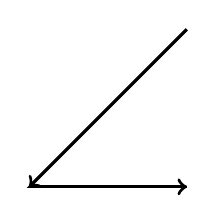
\begin{tikzpicture}

		% define point

		\coordinate (A)  at (2, 2);

		\coordinate (O)  at (0, 0);

		\coordinate (B)  at (2, 0);

		% angle  

		\draw[thick] (A) -- (O) -- (B);

		%\draw pic[draw=black,angle radius=20,angle eccentricity=1.4]

		%{angle = B--O--A};

		%\pic [draw,"$\alpha_1$",angle radius=20,->,angle eccentricity=1.4]

		%  {angle = B--O--A};

		\draw [->, very thick] (2,2) -- (0,0)  node [midway, above] {\scriptsize };

		\draw [->, very thick] (0,0) -- (2,0)  node [midway, above] {\scriptsize };

	\end{tikzpicture}

	\captionof{figure}{\textbf{Slope Gesture \cite{Warden:2020}}}

	\label{fig:Slope Gesture}

\end{figure}



Data collection involves controlled experiments where users perform gestures repeatedly, with sensors synchronized to ensure temporal alignment. Preprocessing includes timestamp alignment, noise filtering (e.g., low-pass filtering for IMU data), and image stabilization for camera data. Academic studies on IMU-based gesture recognition emphasize the importance of multimodal data fusion, combining IMU and vision data using techniques like Kalman filtering or sensor fusion algorithms to enhance accuracy \cite{Starlino:2011,Din:2020}.



\section{Data Quantity}

The quantity of data required for training depends on the gesture complexity, model architecture, and device constraints. For TinyML on the Pico4ML-Pro, datasets typically comprise 500–2,000 samples per gesture (e.g., 1,000 samples each for "Wings," "Ring," and "Slope" gestures) to train lightweight models like quantized convolutional neural networks (CNNs), decision trees, or k-nearest neighbors (k-NN). Each sample includes IMU time-series data (e.g., 100 time steps of 3D acceleration and gyroscope readings) and corresponding camera frames (e.g., 10–20 frames per gesture). Insufficient data can lead to overfitting, while excessive data exceeds the Pico4ML-Pro’s memory limits (264 KB SRAM), necessitating data augmentation (e.g., adding noise, scaling, or rotating samples) and efficient data compression techniques \cite{Sadiq:2022, Li:2020}. Research on edge ML suggests that transfer learning from pre-trained models can reduce data requirements, leveraging generic motion patterns for fine-tuning on specific gestures \cite{Bistrov:2012}.



\section{Data Quality}

Ensuring high data quality is paramount for reliable gesture recognition. IMU data is susceptible to noise from drift, vibration, and quantization errors, while camera data faces challenges like lighting variations, motion blur, and background clutter. Preprocessing techniques include:



\begin{itemize}

	\item \textbf{IMU Data}: Applying Kalman filters or complementary filters to mitigate drift and noise, normalizing acceleration and angular velocity to a common scale, and compensating for temperature-induced errors \cite{Bishop:1995,Bistrov:2012}.

	\item \textbf{Camera Data}: Using image stabilization, edge detection (e.g., Canny edge detection), and background subtraction to isolate hand movements, followed by feature extraction (e.g., optical flow or HOG descriptors) \cite{Garcia:2019}.

\end{itemize}



Data quality is further enhanced by controlling experimental conditions (e.g., consistent lighting, minimal background noise) and accounting for inter-user variability, such as differences in hand size, speed, and motion style. Robustness testing, as described in studies on wearable gesture systems, involves evaluating performance across diverse users and environments \cite{Perumandla:2021, Gupta:2022}.



\section{Data Relevance}

Data relevance ensures that only features critical for gesture classification are retained, minimizing computational overhead on the Pico4ML-Pro. For IMUs, relevant features include acceleration magnitude, angular velocity, and motion trajectories (e.g., extracted via dynamic time warping or Fourier transforms). For camera data, relevant features include hand position, motion boundaries, and spatial patterns (e.g., extracted via CNNs or SIFT descriptors). Irrelevant data—such as background noise, static postures, or sensor artifacts—are filtered out using dimensionality reduction techniques like principal component analysis (PCA) or t-SNE, and domain-specific feature selection based on gesture kinematics \cite{Wang:2019, Park:2014}. This approach aligns with research on feature engineering for edge ML, emphasizing efficiency and interpretability \cite{Coogan:2006}.



\section{Outliers}

Outliers in gesture data can arise from erratic movements (e.g., unintended hand jerks during a "Slope" gesture), sensor malfunctions (e.g., IMU drift), or user errors. These are identified using statistical methods such as Z-scores, interquartile range (IQR) analysis, or Mahalanobis distance, and mitigated through robust preprocessing or outlier-robust algorithms. For instance, robust PCA or median filtering can handle outliers in IMU data, while visual outliers (e.g., occluded hand movements) are addressed using motion tracking algorithms like Lucas-Kanade optical flow \cite{Park:2014, Li:2020}. On the Pico4ML-Pro, lightweight outlier detection is preferred, such as simple thresholding or one-class SVMs, to maintain computational efficiency \cite{Garcia:2019,Bishop:1995}.



\section{Anomalies}

Anomalies, such as unexpected gestures (e.g., a sudden erratic motion during a "Ring" gesture) or sensor failures, must be detected to ensure system reliability. Anomaly detection techniques include clustering (e.g., k-means on motion features), autoencoders (for reconstructing normal gesture patterns), or statistical models (e.g., Gaussian mixture models). On the Pico4ML-Pro, these methods are optimized for low memory and power usage, using quantized models or rule-based systems to identify deviations from trained gesture patterns. Research on anomaly detection in edge devices emphasizes the importance of real-time processing and false-positive minimization, ensuring the Magic Wand remains responsive and accurate \cite{Gupta:2022, Perumandla:2021, VboxAutomotive:2023}.



\section{TinyML and ML on Edge Devices}

TinyML, a paradigm for deploying ML on ultra-low-power devices, is central to the Magic Wand’s functionality. The Arducam Pico4ML-Pro’s RP2040 microcontroller supports lightweight models like quantized CNNs, decision trees, or k-NN, trained offline on high-performance systems and deployed on the edge. These models are optimized using techniques such as weight pruning, quantization (e.g., 8-bit or 4-bit integers), and model compression (e.g., TensorFlow Lite for Microcontrollers) to fit within the device’s 264 KB SRAM and 2 MB flash memory \cite{Banerjee:2023, Sadiq:2022}. Inference is performed in real-time, achieving latencies of 10–50 ms per gesture, depending on model complexity and sensor input. ML on edge devices enables offline processing, preserving user privacy, reducing power consumption (typically <100 mW), and eliminating cloud dependency, making it ideal for portable applications like the Magic Wand \cite{Wang:2019, RobotShop:2023}.

  















